\documentclass[hyperref={pdfpagelabels=false}]{beamer}
\usepackage{lmodern}
\usetheme{CambridgeUS}

\usepackage[english,brazilian]{babel}
\usepackage{multicol}
\usepackage{textcomp}
\usepackage[alf]{abntex2cite}
\usepackage[utf8]{inputenc}
\usepackage[T1]{fontenc}

\title{Sistemas de Equações Lineares - Aplicações}  
\author[Matheus Pimenta]{Matheus Pimenta} 
\institute[UTFPR-CP]{\normalsize Universidade Tecnológica Federal do Paraná \\
	Câmpus Cornélio Procópio
} 
\date{Abril de 2019} 
\begin{document}
	
\begin{frame}
\titlepage
\end{frame} 


%\begin{frame}
%\frametitle{Table of contents}
%\tableofcontents
%\end{frame} 


\section{Programação Linear} 


\begin{frame}
\frametitle{Definições} 
\begin{itemize}

	\item Uma função é \emph{linear} quando envolve apenas constantes e termos com variáveis de primeira ordem. \pause
	\item As variáveis são \emph{contínuas} quando podem assumir quaisquer valores em um intervalo de números reais. \pause
	\item Seja $X$ um conjunto de pontos $X \subset \mathbb{R}^n$ qual quer para todo $x = (x_1,x_2,\dots,x_n) \in X$, existem $a_i$ e $b_i$, com pelo menos um $a_i$ não nulo $$a_1x_1a_2x_2+\dots+a_nx_n=b$$ é um hiperplano em $\mathbb{R}^n$. \pause
	\item Em $\mathbb{R}^n$, um semiespaço é a região de um dos lados de um hiperplano. Em outras palavras, são os pontos $x$ tais que: $$a_1x_1a_2x_2+\dots+a_nx_n \geq b \text{ ou } a_1x_1a_2x_2+\dots+a_nx_n \leq b$$ para determinados $a_i$ e $b \in \mathbb{R}$.
\end{itemize}
\end{frame}

\begin{frame}
\frametitle{Definições}
\begin{itemize}
	\item As \emph{variáveis de decisão} são as incógnitas, ou valores desconhecidos, que serão determinados pela solução do modelo. Podem ser classificadas de acordo com as seguintes escalas de mensuração: variáveis contínuas, discretas ou binárias. As variáveis de decisão devem assumir valores não negativos. \pause
	\item A \emph{função objetivo} é uma função matemática que determina o valor-alvo que se pretende alcançar ou a qualidade da solução, em função das variáveis de decisão e dos parâmetros, podendo ser uma função de maximização ou de minimização. \pause
	\item As \emph{restrições} podem ser definidas como um conjunto de equações e inequações que as variáveis de decisão do modelo devem satisfazer. As restrições são adicionadas ao modelo de forma a considerar as limitações físicas do sistema, e afetam diretamente os valores das variáveis de decisão. \pause
	\item Solução viável ou factível é aquela que satisfaz todas as restrições do modelo, inclusive as de não negatividade.
\end{itemize}

\end{frame}

\begin{frame}
\frametitle{Teorema}
Se a região viável de um Problema de Programação Linear é não-vazia e limitada, então a função-objetivo atinge tanto um valor máximo quanto um valor mínimo e estes ocorrem em pontos extremos da região viável. Se a região viável é ilimitada, então a função-objetivo pode ou não atingir valores máximo ou mínimo; contudo, se atingir um máximo ou um mínimo, este ocorrerá em pontos extremos.

\begin{figure}[!h]
	\centering
	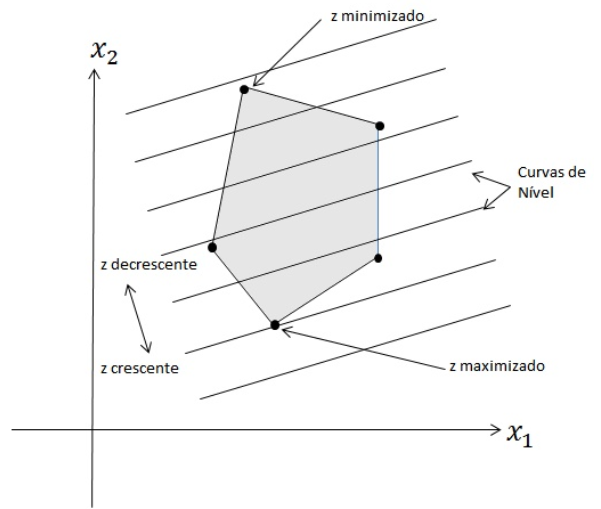
\includegraphics[scale=0.3]{teo}
	\label{teo}
\end{figure}

\end{frame}

\section{Exemplos}

\begin{frame}
\frametitle{Exemplo 01 - Minimização}

Um estudante quer projetar um desjejum com flocos de milho e leite que seja o mais eco-nômico possível. Levando em conta o que ele consegue comer nas suas outras refeições, ele decide que seu café da manhã deveria supri-lo com pelo menos 9 gramas de proteínas, pelo menos um terço da necessidade diária recomendada (VDR) de vitamina D e pelo menos um quarto da VDR de cálcio. Ele encontra as seguintes informações nutricionais nas embalagens do leite e dos flocos de milho:

\begin{table}[h]
	\centering
	\begin{tabular}{ccc}
		\hline
				&	Leite 	&	Flocos de Milho \\
		\hline
		Custo	&	$7,5$ centavos	&	$5,0$ centavos \\
		Proteína &	$4$ gr	&	$2$ gr 	\\
		Vit. D	&	$1/8$ VDR	&	$1/10$ VDR 	\\
		Cálcio	&	$1/6$ VDR	&	Nada	\\
		\hline
	\end{tabular}
\end{table}
A fim de não ter uma mistura muito empapada ou muito seca, o estudante decide limitar--se a misturas que contenham não menos do que 1 e não mais do que 3 xícaras de flocos de milho por xícara de leite. 

\end{frame}

\begin{frame}
\frametitle{Exemplo 01 - Minimização}

Quais quantidades de leite e de flocos de milho ele deve utilizar para minimizar o custo do seu desjejum? \pause

{\bf Formulação Matemática}

Sejam $x_1$ a quantidade de leite utilizada (medida em metade de xícaras) e $x_2$ a quantidade de flocos de milho utilizada (medida em xícaras). Então, sendo $z$ o custo do desjejum (em centavos), podemos escrever as restrições seguintes.

\begin{table}[h]
	\centering
	\begin{tabular}{ll}
		\hline
		Custo do desjejum		&	$z = 7,5x_1 + 5x_2$ \\
		Pelo menos $9$g de Proteínas	&	$4x_1+2x_2\geq 9$ \\
		Pelo menos $1/3$  VDR de vitamina D: &	$\frac{1}{8}x_1+\frac{1}{10}x_2 \geq \frac{1}{3}$ \\
		Pelo menos $1/4$ VDR de cálcio:	&	$\frac{1}{6}x_1 \geq \frac{1}{4}$ \\
		Pelo menos 1 xícara de flocos de milho \\ por xícara (duas  xícaras) de leite: & $\frac{x_2}{x_1}\geq \frac{1}{2}$ ou $x_1-2x_2 \leq 0$ \\
		No máximo 3 xícaras de flocos de milho \\ por xícara (duas $1/2$  xícaras) de leite: & $\frac{x_2}{x_1} \leq \frac{3}{2}$ ou $3x_1 - 2x_2 \geq 0$ \\
		\hline
	\end{tabular}
\end{table}

\end{frame}


\begin{frame}
\frametitle{Exemplo 01 - Minimização}

Como antes, também estamos supondo implicitamente que $x_1 \geq 0$ e $x2 \geq 0$. Assim, a formulação matemática completa do problema é a seguinte: encontrar os valores de $x_1$ e $x_2$ que minimizam
$$z = 7,5x_1 + 5,0x_2$$
sujeito as restrições:
$$4x_1+2x_2\geq 9$$
$$\frac{1}{8}x_1+\frac{1}{10}x_2 \geq \frac{1}{3}$$
$$\frac{1}{6}x_1 \geq \frac{1}{4}$$
$$ x_1-2x_2 \leq 0 $$
$$ 3x_1 - 2x_2 \geq 0 $$
$$ x_1 \geq 0 $$
$$ x2 \geq 0 $$
\end{frame}

\begin{frame}
\begin{figure}[!h]
	\centering
	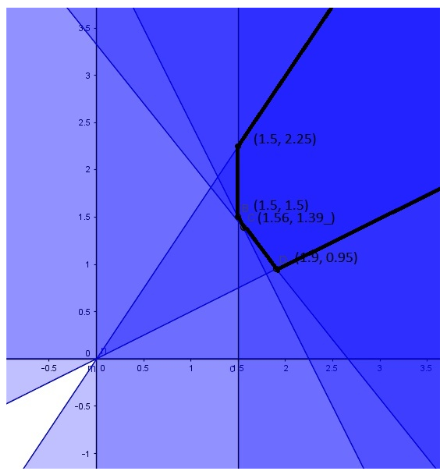
\includegraphics[scale=0.5]{ex1}
	\label{ex1}
\end{figure}
\end{frame}

\begin{frame}
\frametitle{Exemplo 01 - Minimização}

Por ser ilimitada, o Teorema não nos garante que a função-objetivo atinge um valor máximo. De fato, é fácil verificar que, como a região viável contém pontos nos quais ambos $x_1$ e $x_2$ são arbitrariamente grandes e positivos, a função objetivo toma valores arbitrariamente grandes e positivos. Este problema não tem solução ótima. Em vez disto, nós dizemos que o problema tem uma solução ilimitada.

\end{frame}

\begin{frame}
\frametitle{Exemplo 02 - Maximização} 

Um fabricante de bombons tem bombons de chocolate em estoque, sendo 130 kg com recheio de cerejas e 170 kg com recheio de menta. Ele decide vender o estoque na forma de dois pacotes sortidos diferentes. Um pacote contém uma mistura com metade do peso em bombons de cereja e metade em menta e vende por R\$20,00 o quilo. O outro pacote contém uma mistura de um terço de bombons de cereja e dois terços de menta e vende por R\$12,50 o quilo. O vendedor deveria preparar quantos quilogramas de cada mistura a fim de maximizar sua receita?

\end{frame}

\begin{frame}
\frametitle{Exemplo 02 - Maximização}

{\bf Formulação Matemática}

Digamos que $A$ seja a mistura com metade cereja e metade menta e que $x_1$ seja o número de quilogramas dessa mistura que deverá ser preparada. Digamos que $B$ seja a mistura com um terço cereja e dois terços menta e que $x_2$ seja o número de quilogramas dessa mistura que deverá ser preparada. Como o quilograma da mistura $A$ vende por R\$20,00 e o da mistura $B$ vende por R\$12,50, o total $z$ de vendas (em dólares) será:
$$z = 20x_1 + 12,5x_2$$

\end{frame}

\begin{frame}
\frametitle{Exemplo 02 - Maximização}

As restrições serão dadas por:
Como cada quilograma da mistura $A$ contém meio quilograma de bombons de cereja e cada quilograma da mistura $B$ contém um terço de quilograma de bombons de cereja, o número total de quilogramas de bombons de cereja usados em ambas misturas é:
$$\frac{1}{2}x_1 + \frac{1}{3}x_2$$

Analogamente, como cada quilograma da mistura $A$ contém meio quilograma de menta e cada quilograma da mistura $B$ contém dois terços de quilograma de menta, o número total de quilogramas de bombons de menta usados em ambas misturas é:
$$\frac{1}{2}x_1 + \frac{2}{3}x_2$$
\end{frame}

\begin{frame}
\frametitle{Exemplo 02 - Maximização}
Como o fabricante pode usar, no máximo, $130$ quilogramas de bombons de cereja e $170$ quilogramas de bombons de menta, devemos ter:
$$\frac{1}{2}x_1 + \frac{1}{3}x_2 \leq 130$$
$$\frac{1}{2}x_1 + \frac{2}{3}x_2 \leq 170$$

E como $x_1$ e $x_2$ devem ser somente positivas vale:
$$x_1 \geq 0$$
$$x_2 \geq 0$$
\end{frame}

\begin{frame}
\frametitle{Exemplo 02 - Maximização}
Assim, a formulação matemática completa do problema é a seguinte: encontrar os valores de $x_1$ e $x_2$ que maximizem:
$$z = 20x_1 + 12,5x_2$$
sujeito as restrições
$$\frac{1}{2}x_1 + \frac{1}{3}x_2 \leq 130$$
$$\frac{1}{2}x_1 + \frac{2}{3}x_2 \leq 170$$
$$x_1 \geq 0$$
$$x_2 \geq 0$$


\end{frame}


\begin{frame}
\frametitle{Exemplo 02 - Maximização}


\begin{figure}[!h]
	\centering
	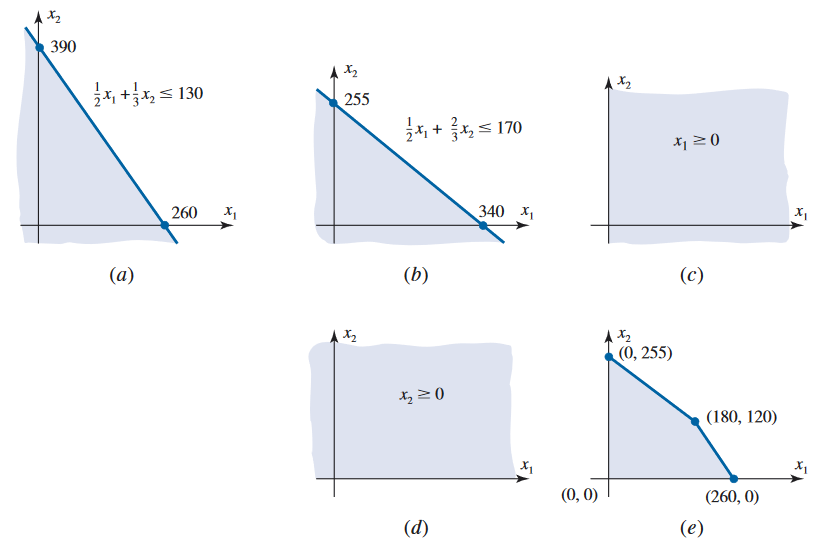
\includegraphics[scale=0.5]{ex2}
	\label{ex2}
\end{figure}

\end{frame}

\begin{frame}
\frametitle{Exemplo 02 - Maximização}

Pode ser mostrado que a região viável de um Problema de Programação Linear tem uma fronteira que consiste de um número finito de segmentos de retas. Uma região viável é dita limitada se puder ser englobada num círculo suficientemente grande; caso contrário, ela é ilimitada.

\pause

Os pontos de fronteira de uma região viável que são intersecções de dois segmentos de retas de fronteira, são chamados pontos extremos.(Também são chamados pontos de esquina ou de vértice.)

\pause

Em nosso exemplo, são os seguintes pontos:
$$ (0,0), (0,255), (180,120), (260,0) $$


\end{frame}


\begin{frame}
\frametitle{Exemplo 02 - Maximização}

A região de análise é uma região limitada, logo pelo Teorema, a função objetivo atinge máximo e mínimo nesta região.

Os valores de extremo da função objetivo é dada pela Tabela:
\begin{table}[h]
	\centering
	\begin{tabular}{cc}
	\hline
	Ponto Extremo		&	Valor de $z$ 	\\
	\hline
	$(0,0)$		&	$0$	\\
	$(0,255)$	&	$3187,50$	\\
	$(180,120)$	&	$5100$	\\
	$(260,0)$	&	$5200$	\\
	\hline
	\end{tabular}
\end{table}

\pause

Nós vemos que o maior valor de $z$ é $5200,00$ e a correspondente solução ótima é $(260,0)$. Assim, o fabricante de balas atinge um máximo de $R\$5.200,00$ de vendas quando ele produz $260$ quilos da mistura $A$ e nada da mistura $B$.

\end{frame}
















\end{document}

